\chapter{Empirical Study of Data Breaches \\ and an Anatomy of MitB Malware}
\label{chp3::breaches}

\vspace*{-0.5cm}
We conduct an empirical analysis of data and user secret breaches to understand how secrets are compromised and leaked in the wild. This chapter collects and analyses 60 web security and data breaches from 2020, examining their causes and impact. We establish an evidence-based foundation that informs our subsequent chapters on the use of secrets (such as passwords), client and server-side protections, and vulnerabilities.

\vspace*{-0.5cm}
\section{Introduction}
\label{sec::chp3::introduction}

Collecting and analysing data breaches enables us to understand the threat vectors and actors, facilitating vicarious learning for other observers, who can then apply these insights to better protect themselves, especially given that organisations are primarily responsible for protecting user secrets. Two main ways of obtaining insights and statistics on data breaches are: 1) when a breach is reported by the victim organisation to a regulatory body, such as the UK's Information Commissioner's Office (ICO); or 2) when breaches are discovered online and subsequently reported by journalists or experts. Self-reported incidents rarely provide detailed accounts of the attack; the most useful information is often gleaned from journalist reports or white-hat hackers. Thus, in this chapter, we will collect and analyse open-source reports and go deeper than regulatory reports. We will draw insights from case studies and post-mortem reports.

We aim to understand MitB malware in more detail. It has been underreported, especially given that it operates silently and exfiltrates the most valuable user secrets, such as complete banking information. Additionally, some of the most prominent data breaches and cyber incidents have been MitB-based attacks; examples include the British Airways~\cite{klijnsma_british_2018} and Ticketmaster case~\cite{corfield_ticketmaster_nodate}. Section~\ref{sec::chp3::mitb} provides a detailed exposition of MitB malware.

The literature on this topic of understanding breaches in detail is sparse. The work of Saleem~\etal~\cite{saleem_sok_2020} is most similar to our intent; they conduct a systematic analysis and workflow of ten data breaches between 2013 and 2014. Bilge~\etal~\cite{bilge_before_2012} perform a similar systematic analysis but focus on zero-day attacks between 2008 and 2011. Attack2Vec~\cite{shen_attack2vec_2019} formalises attacks in the CVE type and time---a useful method for understanding the evolution of an attack. Thomas~\etal~\cite{thomas_data_2017} study the data and consequences of breaches themselves, including credentials, keyloggers, and phishing kits. Abramova~\etal~\cite{abramova_anatomy_2023} analyse a specific breach and subsequently conduct a survey on user behaviour and attitudes towards data breaches.

We will use the cost of data breaches and their impact on businesses to motivate the need to understand and mitigate data breaches. In 2019--2020, UK data controllers reported (via the UK's ICO\footnote{Information Commissioner's Office}) a total of \num{2\,353} cyber incidents~\cite{ico_historical_2020}, as shown in Figure~\ref{fig:1920pie}. In Q2 of 2020–-2021 (July 2020 to October 2020), UK data controllers reported \num{737} cases~\cite{ico_historical_2020}, which equates to 30\% of the previous year's total cases. This increase in attacks is straining organisations, especially those that lack adequate resources to protect themselves. Some businesses believe they do not receive sufficient guidance~\cite{furdui_502_2019}. These cyber incidents impose significant costs on organisations. Complex regulatory landscapes and emerging attack vectors, such as ransomware, make predicting these costs difficult. IBM reports that the average cost of a data breach is \$3.86 million~\cite{ibm_security_ibm-2020_2020}, and it takes an average of 280 days to resolve a data breach. There are direct costs, including legal fees and regulatory fines, as well as indirect costs, such as customer loss, reduced productivity, and other opportunity costs. A third of UK businesses lost customers~following~a~security~breach~\cite{furdui_502_2019}.

\begin{figure}[t]
\centering
\textbf{UK Cyber Incidents 2019-20}\par
\textbf{Total Reported Incidents: 2,353}\par\medskip
\begin{tikzpicture}
    \pie[radius=1.75]{49/Phishing ,25/{Unauthorised access} ,9/Other ,7/Ransomware ,4/Malware ,4/Misconfigs*, 1/Brute Force}
\end{tikzpicture}
\caption{Reported cyber incidents to UK’s Information Commissioner’s Office from April 2019 to April 2020 \cite{ico_historical_2020}. These are reported incidents by data controllers. Does not reflect total incidents. \* Hardware and Software Misconfiguration}
\label{fig:1920pie}
\end{figure}


\section{Method}
\label{sec::chp3::method}

This method facilitates the collection of reported data breaches online and their categorisation. Our goal is to understand the attack vectors and classify them accordingly. We gathered data from open-source news reports, focusing on the attack method, number of records breached, data types, and other relevant metadata.

\paragraph*{Attack Classification.} We categorised the attacks using the following taxonomy:
\begin{itemize}
\item \textbf{Man-in-the-Browser (MitB)}: Code injection attacks or malicious third-party scripts executing on the client or browser in order to exfiltrate user data as they are being entered. 

\item \textbf{Phishing}: Social engineering techniques used to trick users into revealing sensitive information or granting access to a system, often through spoofed emails or fake websites.
\item \textbf{Unprotected Database}: Misconfigured or unsecured databases or storage systems (e.g., AWS S3 buckets) that are publicly accessible without proper access controls.

\item \textbf{Credential Stuffing Attack (CSA)}: Automated injection of compromised credentials into login forms to gain unauthorised access to user accounts.

\item \textbf{Unknown}: Incidents where the attack method could not be determined based on available open-source information.

\item \textbf{Other}: Attacks not fitting into the above categories, such as SQL injection (SQLI), supply chain attacks, or exploitation of insecure code.
\end{itemize}
\paragraph*{Data Categories.} We classified the compromised data into the following categories:
\begin{itemize}
\item \textbf{Personally Identifiable Information (PII)}: Data that can be used to uniquely identify an individual, such as name, address, social security number, or biometric data.
\item \textbf{Healthcare}: Sensitive medical information, including patient records, medical history, or insurance details.
\item \textbf{Financial}: Full or partial bank card information, such as credit card numbers, expiration dates, or CVV codes.
\item \textbf{Authentication}: User credentials, such as email addresses, usernames, or passwords (hashed or plaintext).
\end{itemize}


\section{Results and Evaluations}
\label{sec::chp3::results}

Table~\ref{table:main} summarises our results. We analysed sixty attacks that were reported in 2020. We investigated each attack and data breach and came to a conclusion on the cause and type of attack. Our data sources were open-source material. This section follows the table structure in Table~\ref{table:main}---we discuss the results in each category.

\setlength\dashlinedash{0.2pt}
\setlength\dashlinegap{1.5pt}
\setlength\arrayrulewidth{0.4pt}


\begin{table*}
\scriptsize
\centering
\caption{Analysis of 60 open source reports of data breaches and web attacks categorised based on method of attack.}
\label{table:main}
    \setlength\tabcolsep{3pt} % default value: 6pt
    {\renewcommand{\arraystretch}{0.8}% for the vertical padding
\begin{tabular}{rlp{1cm}cccccl}
\toprule
\rowcolor{white}
& & & & \multicolumn{2}{c}{\textbf{Incident Date}} & & \\
& Victim & Records & Data & From & To & News Date & Src \\
\toprule
\multicolumn{2}{l}{ \textbf{Credential Stuffing Attack} } & & & & & \multicolumn{2}{c}{ Total: 4 } \\
\hline
1 & US--\textbf{J.CREW} & n/a & PII, \$, Sensitive activity & n/a & Apr '19 & Mar & \cite{whittaker_jcrew_2020} \\
\hdashline
2 & US--\textbf{Amtrak} & n/a & PII & n/a & Apr & Jun & \cite{osborne_amtrak_2020,mares_amtrak_2020} \\
\hdashline
3 & US--\textbf{Spotify} & 0.30 & PII & n/a & Nov & Nov & \cite{moore_thousands_2020} \\
\hdashline
4 & US--\textbf{Zoom} & 0.50 & PII & n/a & Apr & Apr & \cite{abrams_over_2020} \\
\hdashline
\multicolumn{2}{l}{ \textbf{Man-in-the-Browser} } & & & & & \multicolumn{2}{c}{ Total: 7 } \\
\hline
5 & US--\textbf{Warner Music Group} & n/a & PII, \$ & Apr & Aug & Sept & \cite{broersma_warner_2020} \\
\hdashline
6 & GB--\textbf{Sweaty Betty} & n/a & PII, \$ & Nov '19 & Nov '19 & Dec '19 & \cite{noauthor_sweaty_2019,abrams_uk_2019} \\
\hdashline
7 & US--\textbf{Claire's} & n/a & PII, \$ & Apr & Jun & Jun & \cite{sandle_claires_2020} \\
\hdashline
8 & US--\textbf{Boom! Mobile} & n/a & PII, \$ & n/a & Oct & Oct & \cite{osborne_boom_2020} \\
\hdashline
9 & US--\textbf{Hanna Andersson} & 0.20 & PII, \$ & 09 '19 & 11 '19 & Jan & \cite{de_la_torre_hanna_2020,towsend_hanna_2020} \\
\hdashline
10 & US--\textbf{JM Bullion} & n/a & PII & Feb & Jul & Nov & \cite{kovacs_gold_2020} \\
\hdashline
11 & US--\textbf{San Francisco Int Airport} & n/a & Auth & n/a & Apr & Apr & \cite{abhliash_breaking_2020} \\
\hdashline
12 & \textbf{Cardbleed - Int} & n/a & PII, Auth, \$ & Sept & Sept & Sept & \cite{team_sansec_cardbleed_2020} \\
\hdashline
\multicolumn{2}{l}{ \textbf{Phishing} } & & & & & \multicolumn{2}{c}{ Total: 5 } \\
\hline
13 & US--\textbf{Tufts Health Plan \& EyeMed} & 0.06 & PII & July & Nov & Dec & \cite{noauthor_tufts_nodate} \\
\hdashline
14 & US--\textbf{Twitter} & 130 Accounts & Auth, Msg & n/a & Aug & Aug & \cite{noauthor_teen_2020} \\
\hdashline
15 & US--\textbf{Imperium Health} & 0.14 & PII, PHI & Apr & Apr & Sept & \cite{hippa_journal_phi_2020} \\
\hdashline
16 & US--\textbf{Ambry Genetics} & 0.23 & PII & Jan & Jan & Apr & \cite{bizga_medical_2020} \\
\hdashline
17 & US--\textbf{Beaumont Health} & 0.12 & PII, Health & May & Jun & Jul & \cite{noauthor_6000_2020} \\
\hdashline
\multicolumn{2}{l}{ \textbf{Ransomware} } & & & & & \multicolumn{2}{c}{ Total: 3 } \\
\hline
18 & US--\textbf{Magellan Health} & 1.70 & PII, Auth & Apr & Apr & May & \cite{davis_ransomware_2020} \\
\hdashline
19 & DE--\textbf{Fresenius Group} & n/a & System & n/a & May & May & \cite{krebs_europes_2020} \\
\hdashline
20 & US--\textbf{Barnes \& Noble} & n/a & PII, Sensitive activity & n/a & Oct & Oct & \cite{abrams_barnes_2020} \\
\hdashline
\multicolumn{2}{l}{ \textbf{Unknown} } & & & & & \multicolumn{2}{c}{ Total: 10 } \\
\hline
21 & US--\textbf{Drizly} & 2.50 & PII, \$ & n/a & Feb & Jul & \cite{whittaker_alcohol_2020} \\
\hdashline
22 & US--\textbf{Quidd} & 4.00 & PII, Auth & n/a & Oct & Mar & \cite{noauthor_nearly_2020} \\
\hdashline
23 & US--\textbf{MGM Resorts} & 142 & PII & n/a & Jul & Jul & \cite{noauthor_mgm_2020} \\
\hdashline
24 & JP--\textbf{Nintendo - JP} & 0.30 & PII, \$ & n/a & Apr & Jun & \cite{liao_nintendo_2020} \\
\hdashline
25 & US--\textbf{Dental Care Alliance} & 1.00 & PII, Sensitive info & Sept & Oct & Dec & \cite{noauthor_dental_2020} \\
\hdashline
26 & US--\textbf{Wishbone} & 40.00 & PII, Auth & Jan & May & May & \cite{cimpanu_hacker_2020} \\
\hdashline
27 & HR--\textbf{Mathway} & 25.00 & PII, Auth & n/a & Jan & May & \cite{cimpanu_25_2020} \\
\hdashline
28 & US--\textbf{Minted} & 5.00 & PII, Auth & May & May & May & \cite{abrams_minted_2020} \\
\hdashline
29 & US--\textbf{Chowbus} & 0.80 & PII, & n/a & Oct & Oct & \cite{abrams_chowbus_2020} \\
\hdashline
30 & GB--\textbf{EasyJet} & 9.00 & PII, \$ & April & April & May & \cite{wakefield_easyjet_2020} \\
\hdashline
\multicolumn{2}{l}{ \textbf{Unsecured Database} } & & & & & \multicolumn{2}{c}{ Total: 19 } \\
\hline
31 & US--\textbf{Pray.com} & 10.00 & PII, Sensitive activity & n/a & n/a & Nov & \cite{seals_good_2020} \\
\hdashline
32 & US--\textbf{Paay} & 2.50 & Payment Info & Apr & Apr & Apr & \cite{riley_25m_2020} \\
\hdashline
33 & US--\textbf{Clubillion} & >1 & PII, Activity & n/a & Apr & Apr & \cite{noauthor_report_2020} \\
\hdashline
34 & NL--\textbf{Pfizer (EMA)} & n/a & Docs & n/a & n/a & Dec & \cite{noauthor_pfizerbiontech_2020} \\
\hdashline
35 & US--\textbf{Estee Lauder} & 440 & PII, Activity & n/a & Jan & Feb & \cite{paganini_440m_2020} \\
\hdashline
36 & US--\textbf{Whisper} & 900 & PII & 2012 & Mar & Mar & \cite{osborne_whisper_2020} \\
\hdashline
37 & US--\textbf{MyCastingFile.com} & 0.26 & PII, Sensitive info & n/a & Apr & Jul & \cite{osborne_us_2020} \\
\hdashline
38 & US--\textbf{PhotoSquared} & 0.10 & PII, Sensitive info & Nov & Jan & Feb & \cite{muncaster_photosquared_2020} \\
\hdashline
39 & US--\textbf{Ancestry.com} & 0.06 & PII, Sensitive info & n/a & Jul & Jul & \cite{montalbano_leak_2020} \\
\hdashline
40 & MY--\textbf{123RF} & 8.30 & PII, Auth & n/a & Oct & Nov & \cite{noauthor_hackers_2020} \\
\hdashline
41 & US--\textbf{Fragomen, Del Rey, Bernsen \& Loewy} & -- & PII & n/a & n/a & Oct & \cite{noauthor_fragomen_2020} \\
\hdashline
42 & US--\textbf{Key Ring} & 14.00 & PII & n/a & Jan & Feb & \cite{coble_key_2020} \\
\hdashline
43 & GB--\textbf{Virgin Media} & 0.90 & PII & n/a & Mar & Mar & \cite{cimpanu_virgin_2020} \\
\hdashline
44 & US--\textbf{U.S. Marshals Service} & 0.39 & PII & n/a & Dec & May & \cite{cimpanu_us_2020} \\
\hdashline
45 & US--\textbf{Vertafore} & 27.70 & PII & Mar & Aug & Nov & \cite{cimpanu_info_2020} \\
\hdashline
46 & US--\textbf{CouchSurfing} & 17.00 & PII & n/a & Jul & Jul & \cite{cimpanu_couchsurfing_2020} \\
\hdashline
47 & US--\textbf{Broadvoice} & 350.00 & PII, Sensitive Activity, Msg & n/a & Oct & Oct & \cite{noauthor_broadvoice_2020} \\
\hdashline
48 & US--\textbf{Avon} & 19.00 & PII & n/a & Jun & Jul & \cite{muncaster_cosmetics_2020} \\
\hdashline
49 & CN--\textbf{Peekaboo Moments} & n/a & PII, Media & n/a & Jul & Jul & \cite{mares_millions_2020} \\
\hdashline
\multicolumn{2}{l}{ \textbf{Other} } & & & & & \multicolumn{2}{c}{ Total: 11 } \\
\hline
50 & US--\textbf{Slickwraps} & 0.85 & PII, HR, Sys & Feb & Feb & Feb & \cite{lynx0x00_i_2020} \\
\hdashline
51 & US--\textbf{BlueLeaks (Netsential)} & 0.70 & PII, \$, Activity & n/a & Jun & Jun & \cite{krebs_blueleaks_2020} \\
\hdashline
52 & US--\textbf{Beaumont Health} & 0.00 & PII, Health & Feb & Oct & Jan & \cite{noauthor_6000_2020} \\
\hdashline
53 & US--\textbf{Dickey's BBQ} & 3.00 & \$ & May '19 & Sep '20 & Oct & \cite{krebs_breach_2020} \\
\hdashline
54 & US--\textbf{Health Share of Oregon} & 0.65 & PII++ & n/a & Jan & Feb & \cite{osborne_health_2020} \\
\hdashline
55 & US--\textbf{Walgreens} & <10 & PII & May & Jun & Jul & \cite{bizga_walgreens_2020} \\
\hdashline
56 & ES--\textbf{Freepik} & 8.30 & Auth & n/a & Aug & Aug & \cite{freepik_statement_2020} \\
\hdashline
57 & US--\textbf{Mashable.com} & n/a & PII, HR & n/a & Nov & Nov & \cite{waqas_shinyhunters_2020,mashable_notice_2020} \\
\hdashline
58 & US--\textbf{Dave Mobile Banking App} & 7.50 & PII, Auth & n/a & Jun & Jul & \cite{cimpanu_tech_2020} \\
\hdashline
59 & US--\textbf{General Electric} & 0.28 & PII & Feb & Feb & Mar & \cite{spadafora_general_2020} \\
\hdashline
60 & IL--\textbf{Promo.com} & 22.00 & PII & n/a & Jul & Jul & \cite{abrams_promocom_2020} \\
\bottomrule
\end{tabular}


} % vertical padding
\end{table*}


\subsection{Credential Stuffing Attacks}
\label{sec::chp3::csa}

Credential Stuffing Attack (CSA) is the consequence of password re-use across web applications. The insights here are limited due to the reporting nature of these attacks and most often the organisations themselves were not aware of the attack. We expect CSA attacks to keep growing as more credentials are leaked online.


\subsection{Man-in-the-Browser}
\label{sec::chp3::mitb}

\begin{figure}
    \centering
    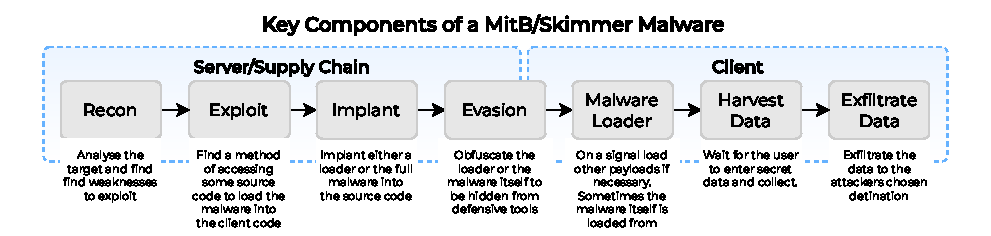
\includegraphics{figs/breaches_chapter3/mitb_components.pdf}
    \caption{Graphical representation of the Man-in-the-Browser (MitB) malware components. Based on the observed MitB-based cyber incidents, we divide the malware into seven ordered components. The taxonomy is based on key components that enable the success or the failure of the malware. For example, when the data is being exfiltrated, the attacker has to overcome Content Security Policy (CSP). \srcOwnFig}
    \label{chp3::fig::mitb-components}
\end{figure}

The Man-in-the-Browser (also known as \textit{form grabbers}, \textit{skimmers}, or \textit{magecart-style attacks}) incidents were highly sophisticated and targeted attacks. Our first insight is on the anatomy of a MitB malware: we divide the malware into six key components, as seen in Figure~\ref{chp3::fig::mitb-components}. We should note here that we are focusing on a variant of a MitB malware that originates from a compromised server. MitB malware can also originate from a compromised third-party script or the user's device itself could be compromised.

The suggested components of a Man-in-the-Browser (MitB) malware can be best explained through the life-cycle of such an attack, as shown in Figure~\ref{chp3::fig::mitb-components}.The attacker would begin by understanding the target, where the majority of them are e-commerce platforms or applications with a payment gateway. These applications are most valuable because of the frequency at which users enter their banking details (which are typically not stored in full on the server). The attacker would conduct a reconnaissance (recon) to find a route into the server (or to conduct a supply chain attack). E-commerce platforms that have poor admin security are easy targets. Once the server is \textit{exploited}, the attacker would implant their malware or loader into the application. Their choices here will determine how well they would be able to \textit{evade} discovery. Their choice here also depends on the level of effort put into tailoring their malware for a specific target. Some attackers choose to use a \textit{loader} to evade discovery--this loader has a smaller footprint and is timed to load the malware during checkout when the user is entering sensitive data. Next, the attacker needs to \textit{harvest} the user data; they can do this by creating a fake checkout page or grabbing user data from the HTML input fields. Finally, the attacker would \textit{exfiltrate} the data either through the compromised server or through methods such as the image GET request method.


\paragraph{Implant and Evasion Methods} \textit{Implant} refers to where and how a payload is embedded into a target's web application, typically through vulnerabilities in the application's code or configuration. \textit{Evasion} encompasses the techniques used by attackers to avoid detection or prevention mechanisms while carrying out their attacks. Through empirical analysis of real-world attacks, we can better understand the methods devised by attackers and develop more effective defenses for web applications, ultimately improving their security posture.

\begin{itemize}
\item \textbf{Timed\;Response:} When an attacker only activates their malware at a specific point in the user's journey on a website, it is said to be \textit{timed}. An example of this is where an attacker used a malicious icon and favicon website to only deliver malicious content on a checkout page \cite{segura_credit_2020}. This method helps the attacker evade static analysers or methods that do not take the full user journey into account.

\item \textbf{EXIF\;Metadata:}\;Image headers being used to hide malicious credit card skimming JavaScript code. In one example \cite{segura_web_2020}, Malwarebytes Labs show how the copyright field (in the EXIF metadata) was used to transport the obfuscated JavaScript code. This technique allows attackers to bypass content security policies.

\item \textbf{Image:}\;There are multiple examples~\cite{leal_skimmer_2020, segura_criminals_2020} of images being used to hide malicious JavaScript code that is later processed by obfuscated code.

\item \textbf{CSS\;File:}\;Sinegubko~\cite{sinegubko_css-js_2020} demonstrates how attackers conceal malicious JavaScript code within \texttt{.css} files. By exploiting CSS properties like \texttt{content} and \texttt{background-image}, attackers can encode and embed malicious payloads. These payloads are subsequently decoded and executed by the victim's browser when the CSS file is processed, effectively bypassing traditional security controls that focus on JavaScript files.

\item \textbf{Web\;Font:}\;Attackers can embed malicious JavaScript code inside web font files~\cite{martin2022woocommerce}, such as \texttt{.woff} or \texttt{.ttf}, which are then loaded by the target website. When the browser processes these manipulated font files, the malicious code is executed.

\item \textbf{HTML5\;Local\;Storage:}\;Attackers can use HTML5 local storage to persist malicious JavaScript code on the user's browser. This stored code can be later retrieved and executed, even if the user navigates away from the compromised website, allowing the attacker to maintain a persistent presence on the user's system.

\item \textbf{Service\;Worker\;Hijacking:}\;Service workers, a feature of progressive web apps, can be hijacked by attackers to intercept and modify network requests. By registering a malicious service worker, attackers can steal sensitive information, such as login credentials or credit card details, as they are transmitted between the user's browser and the web server.

\item \textbf{Polyglot\;Files:}\;Attackers can create polyglot files, which are files that are valid in multiple formats. For example, an attacker could create a file that is both a valid image and a valid JavaScript file. When this file is loaded by the browser, the malicious JavaScript code is executed.
\end{itemize}

\paragraph{Exfiltration:} This is the method attackers employ to transmit harvested data to their controlled infrastructure. The process presents several technical challenges, particularly bypassing security mechanisms like Content Security Policy (CSP). A common exfiltration technique involves disguising stolen data as parameters in image GET requests, making the data transfer appear as legitimate image loading. More sophisticated approaches leverage third-party infrastructure and messaging platforms' APIs, such as Telegram or Google App Script, to establish covert communication channels while evading detection. These methods often succeed because they utilize trusted services and legitimate APIs that are typically allowed in security policies.

\begin{itemize}
\item \textbf{Image GET Request:} Attaching the harvested data as URL parameters in a GET request for an image hosted on the attacker's server.
\item \textbf{WebSocket Exfiltration:} Establishing a WebSocket connection to the attacker's server and transmitting the data over this channel.
\item \textbf{DNS Tunneling:} Encoding the data within DNS queries and responses, allowing the data to bypass firewall restrictions.
\item \textbf{Telegram Bot API:} Leveraging the Telegram Bot API to send the harvested data to a Telegram channel or chat controlled by the attacker.
\item \textbf{Google App Script:} Utilizing Google App Script to exfiltrate data by sending it to a Google Sheet or other Google service controlled by the attacker.
\item \textbf{ICMP Tunneling:} Encapsulating the data within ICMP echo request and reply packets, enabling data transmission through firewalls that allow ICMP traffic.
\end{itemize}

\paragraph{Case Studies:} We have a detailed breakdown of the attack on \textbf{Claire's} and \textbf{Boom! Mobile}. In both of these attack's, the attackers were able to gain full access to the source code on the server and therefore implant their malware. Overview of each of the attacks are as follow.

\begin{itemize}
\item \textbf{Warner Music:} The server was compromised and malicious JavaScript were injected in order to carry out MitB attack.

\item \textbf{JM Bullion}. Same as Warner Music. It took five months for the company to discover the breach and a further three months to alert the effected customers.

\item \textbf{Claire's:} Sansec~\cite{sansec_magecart_2020} indicates that the attackers were able to access the store's source code and manipulate any file. How they were able to access the code is yet unknown. However, it is noted that the stores are hosted on the Salesforce Commerce Cloud (previously known as Demandware). The obfuscated malware was added to the \texttt{app.min.js} file. It uses \texttt{jQuery} functions to attach to the checkout form's button. Once this checkout button is clicked, an image from the attacker's server is loaded into the DOM, and the customer's information is appended to the image file and exfiltrated via a \texttt{GET} request.

\item \textbf{Sweaty Betty:} A UK-based retailer had its source code infiltrated \cite{abrams_uk_2019}. The attacker injected their malware into a \texttt{custom.js} \cite{noauthor_sweaty_2019} file. The store was---like Claire's---ran on Salesforce Commerce Cloud (Demandware) platform. The obfuscated JavaScript code communicated with the following URL. \texttt{https://www.cdcc02.com/widgets/main.js}.

\item \textbf{\ha:} A children's clothing company in the USA also suffered from a MitB attack; the extent of the attack is unknown but the court-filings suggest approximately \num{200000} victims. Sources suggest that the firm was not aware of the attack until law enforcement notified them of the attack; this could be due to victims reporting fraud whom were consequently linked back to \ha. The e-commerce platform that was used was operated by Salesforce~\cite{noauthor_salesforces_2021} (as with \textit{Sweaty Betty} and \textit{Claire's}.) The main lesson here is that even if you outsource the IT operations and platform, there are business, legal and PR consequences to web and data breaches.

\begin{figure}[t]
    \centering
    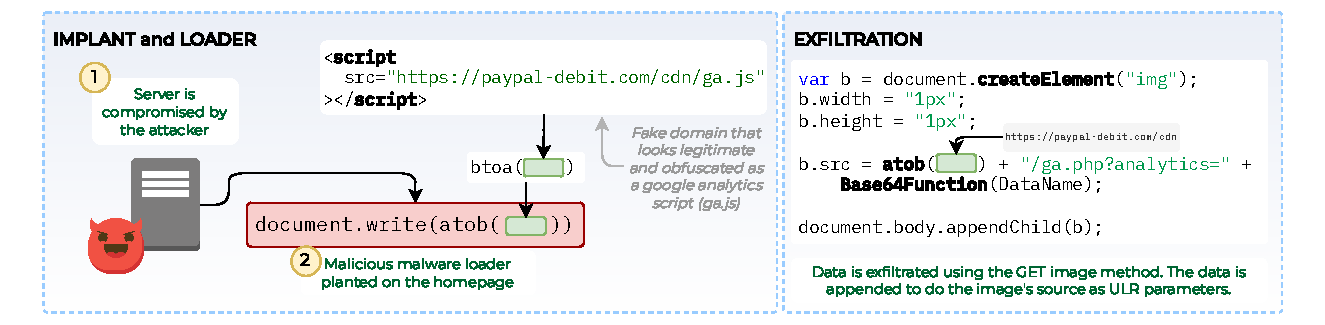
\includegraphics[scale=0.8]{figs/breaches_chapter3/boom_mobile_graphics.pdf}
    \caption{Components of the MitB malware used in the Boom!\;Mobile attack~\cite{team_mobile_2020}. This is a simple example where the attacker is using a fake domain to load the malware from and exfiltrate user's data to. The malware itself is not obfuscated, instead a one line JavaScript loader is used. \srcOwnFig}
    \label{fig:boom-mobile}
\end{figure}

\item \textbf{Boom!\;Mobile:} Malwarebytes Labs report \cite{team_mobile_2020} that a criminal related to the \textit{Fullz House} entity had infiltrated the \texttt{boom.us} site and implanted a MitB malware. Figure \ref{fig:boom-mobile} shows an overview of some of the components of the malware. The attacker had made no attempt at obfuscating much of the source code apart from encoding the URLs using Base64 encoding.

\item \textbf{Cardbleed}. Thousands of Magento e-commerce sites that were running an end-of-life version 1 were exploited over few days. The sites then were injected with MitB malware. The malware exfiltrated payment and personal information to a Moscow-hosted site at \texttt{https://imags.pw/502.jsp}.
\end{itemize}

A limitation of our method is that we have only identified a particular
set of MitB attacks --- attacks that manipulate a site's source code in
the server. This has a bigger reach and probablility of success as
opposed to malware that infects individual end-user devices.

\noteBox{Opportunity: MitB Defence}{%
    \noindent\textbf{Circumventing the threat:} Can we circumvent the threats even if a website or device is compromised? \formless (Chapter \ref{chp::formless} and \fun{Fidelis}~\cite{eskandarian_fidelius_2019} provide some evidence that we can circumvent threats originating from malicious frontends or malicious devices.
    
    \vspace{0.5em}
    \noindent\textbf{Provenance:} Majority of the MitB attacks in Table~\ref{table:main} begun with the attackers gaining access to the source code. Therefore, testing the code-base and understanding where the changes are coming from will help mitigate risks. Tracking unwarranted code insertions through the analysis of its provenance will help fight intruders.
}

\subsection{Unsecured Databases}
\label{sec::chp3::unsecured-db}

An array of unsecured databases and repeated successful attacks imply a poor information security culture. Culture is a set of behaviours, and certain behaviours are necessary to ensure the smooth and secure continuation of any operation. The incidents at Beaumont Health led to attackers gaining access to email accounts, with breaches occurring twice within months. The key takeaway is the need to foster a security-aware culture. Government-backed schemes such as the UK's Cyber Essentials~\cite{uk_gov_cyber_2018} and CISA in the U.S.A.~\cite{cisa_cyber_2020} provide guidance and certification programmes aimed at building a cyber-aware culture at both industry and economic levels—this awareness must be communicated down to the lowest employee within an organisation. The SABSA Enterprise Security Architecture~\cite{noauthor_sabsa_2020} serves as an example of a guiding framework for developing security architecture at various levels within an organisation.

Building a culture that is information security aware---from the beginning---is your best chance of avoiding cyber attacks. Based on our results, reasons why we believe having the right culture can help are as follows.

\begin{itemize}
\item
  \emph{Training}. Phishing and poor passwords result from either a lack of discipline or insufficient knowledge. Organisations can communicate expected security standards and provide employees with the necessary knowledge to recognise and question poor information security practices. However, it is equally important to enforce these standards to ensure compliance and maintain a secure environment.
\item
  \emph{Behaviour}. The SolarWinds attacks~\cite{fireeye_highly_2020} serve as evidence of poor information security discipline, even when there is awareness of the potential negative consequences of such behaviour. Therefore, fostering a self-reinforcing security culture is essential.
\item
  \emph{Sales and Procurement}. With an information security mindset, your employees will question the security of your potential suppliers.
\end{itemize}

In the UK, 40\% of businesses do not have a response plan to inform customers of a breach~\cite{furdui_502_2019}. Implementing a response plan for security breaches enables businesses to restore full operational capability more quickly.

\noteBox{Opportunity: Out-of-band Devices and Zero-Storage Policy}{%
\noindent We can use out-of-band devices to transact secrets and sensitive information within self-contained and secure containers. Consider payment data: web applications typically store only a subset of payment information to protect users while maintaining application usability. However, we can eliminate the need for this approach and its associated risks by enabling users to transact their secrets using another device, such as a mobile phone. Through out-of-band transactions, we can preserve both user experience and security. Additionally, segregating codebases minimises the impact of breaches---a compromised frontend will no longer pose a direct threat to the user. This approach also eliminates the need for users to repeatedly re-enter their~financial~details.
}


\section{Opportunities}
\label{sec::chp3::opportunities}


\subsection{The Data Security Estimate}

For leaders of organisations, the security field can be daunting. Whilst they can get help in the form of consultants, the cash strapped startups and small businesses have to get help elsewhere. So, can we create a framework that can guide an individual in analysing and planning the security of their system and data? Such a framework can provide the following benefits through questioning and hand-railing.

\begin{itemize}
\item
  \emph{Risk:} The framework helps to discover and plan for risks. What
  are the security and data related risks associated to your product,
  business and technology?
\item
  \emph{Systematic Processes:} We have seen that systems are breached
  because of human errors; creating new processes can help minimise
  human errors.
\item
  \emph{Contingency Plans:} Creating what-if scenarios can be helpful in
  thinking through~potential~scenarios.
\item
  \emph{Regulations:} What are the data and web security related
  regulations in my country? And how and when should I interact with
  them?
\item
  \emph{Response Plans}: Do you have a response plan in place to inform
  your customers of a possible data breach? What are the processes in
  plan to deal with a system compromise? How will you ensure business
  continuity?
\end{itemize}

\subsection{PII and Identity}
The majority of incidents in our results led to breaches of personally identifiable information (PII). Compromised organisations, such as \ha, were forced to provide free credit checks and identity protection for the affected customers. This is because customers are at risk of identity theft and fraud. A criminal only needs access to basic personal information—such as name, address, and date of birth—to steal an identity.

We have opportunities in \emph{defending} data from being compromised and \emph{defending} systems and organisations against fraud. Should we rely on \emph{secrecy} and \emph{what-you-know} identity checks? Can legal and decentralised national identity systems neutralise this attack vector? Identity checks, or know-your-customer (KYC) processes, slow down customer onboarding. Therefore, future innovation and research should seek a balance between security and business costs.

%\subsection{PII Uniform Resource Identifier (URI)}
%
%Can the standardisation of storage and communication schemes of PII
%improve security and usability? Our review of the breaches show similar pattern of uncontrolled copies of PII spread across systems with no clear security policies behind them. A PII URI addresses these issues by providing each individual with a resolvable pointer to where their PII is stored and the policies to access it. Standardising this pointer and the surrounding API/policy model aims to improve privacy and usability: people can discover, grant, and revoke access in one place; organisations can separate sensitive PII from operational systems; and sensitive communications move off email into encrypted, auditable channels. Openbanking API is an example of how openining up and standardising the access to financial data leads to economic benefits. Fast Healthcare Interoperability Resources (FHIR).
%
%Mechanically, a relying party receives a `pii:` identifier (or an HTTPS link to `/.well-known/pii`) and resolves it to a small JSON descriptor. That descriptor lists data categories and schemas, API endpoints, the authorization server, supported security profiles, and basic policies (e.g., retention, breach contact). The relying party then asks for a narrow scope with a stated purpose; the user authenticates at their PII provider, grants consent, and a bound, short‑lived token is issued. Only the approved fields are returned—ideally via selective‑disclosure credentials rather than full records—and all access is logged. For sending data, the descriptor can publish an encrypted inbox so PII is exchanged over secure channels instead of email. Standard profiles (OAuth 2.1 or GNAP, FAPI, DPoP or mTLS), consent receipts, webhooks for revocation, and pairwise identifiers provide the security building blocks.
%
%Governance can mirror Open Banking—accredited providers listed in a trust directory, common API and security profiles—but the scope is broader than finance, so privacy controls must be stricter (purpose limitation and minimization by default, pairwise identifiers to prevent correlation, token binding, and timely breach reporting). Incentives are practical: providers can offer “compliance‑as‑a‑service,” relying parties reduce integration and liability costs, regulators get consistent visibility, and users gain portability and control. In the chapters that follow on secrets and protections, this model reduces secret sprawl by replacing emailed PII and static exports with short‑lived, auditable tokens and clear consent, directly addressing the breach causes we observed.
%
%Can the standardisation of storage and communication schemes of PII
%improve security and usability? Such a PII URI can provide the following benefits.
%
%
%\begin{itemize}
%\item \textit{Privacy:} Regulations, such as GDPR in Europe and CCPA in California \cite{noauthor_california_2018}, demand the right for the owner of a dataset to have visibility and access to it. With a URI scheme, there is no ambiguity about how individuals can get access to their data over the web.
%
%\item \textit{Separation of databases:} Organisations can separate PII data from other operational data.
%
%\item \textit{Security:} Creating standardised methods of storing and accessing data can improve security. Furthermore, organisations can separate PII data from other data.
%
%\item \textit{Communication:} PII and other sensitive data are regularly sent over insecure email systems. With a user friendly system built on a URI scheme, one can communicate PII across to other PII storage systems.
%
%\item \textit{Regulation:} This URI scheme and systems can have options to communicate with regulators to report data breaches or create automatic reports. This can improve the relationship between the regulator and the business.
%
%\end{itemize}

\section{Discussion}
\label{sec::chp3::discussion}

%Our intent has been to review web security and data breaches in 2020 to extract lessons learned and identify research opportunities. These incidents have resulted in the exposure of millions of personally identifiable information (PII) records, payment details, and health information. The consequences have affected all stakeholders: customers face identity theft and fraud, organisations suffer business losses, are required to compensate customers, and must contend with regulatory penalties. While the majority of these discussions have been addressed in previous sections, here we will explore the final point—examining the criminals behind these attacks and the limitations of this study.

\textit{Have I Been Pwned?}~\cite{haveibeenpwned} popularised the issue of data breaches and raised awareness of PII and credential leaks. Such awareness has most likely improved the security of many user accounts, as users have been able to change passwords when a leak has occurred. This chapter has, in the same vein, attempted to raise awareness of a large number of breaches in order to understand them and offer solutions on how to defend against them in the future.

We used public news reports instead of dark web publications and breaches because not all breaches are reported in time. Moreover, some breaches are not leaked publicly, so they do not have much presence on the dark web. Our aim has been to understand the nature of the breach rather than the leaked data from the breach.

Our results showed that the Magecart group was behind most of the Man-in-the-Browser (MitB) attacks, and ShinyHunters was behind most of the unknown attacks. This over-reporting of ShinyHunters could be because they openly sell their data online. Their odd behaviour of sometimes making the data available for free adds to the mystery and potential for their name appearing in open-source media. Nevertheless, the evidence shows a network of individuals who have the knowledge, capability, and willingness to carry out these attacks.

The results reinforce the necessity of regulatory oversight: from Virgin Media leaving their marketing database exposed to PhotoSquared storing a vast trove of information in an unprotected AWS storage bucket, numerous organisations have failed to secure their databases and storage instances. The complacent behaviour of many organisations, coupled with a clear lack of learning from past incidents, underscores the need for stringent regulatory~measures.

Reported security breaches covered by various news sources are mostly high-profile cases. As a result, we acknowledge that our dataset represents only a small portion of actual security breaches, making it impossible to correlate our findings with the total number of web attacks and data breaches. Nevertheless, our findings remain valuable given the sample size and the reported incidents. We have been able to extract key lessons and gather useful data for future~research.

The cases we have covered have all been reported through English-speaking media outlets, and all the organisations involved are either European or North American. However, we do not believe that the nature of threats and attack vectors would differ significantly in other countries. Moreover, the reliance on publicly reported incidents creates a significant selection bias towards organisations that either voluntarily disclosed breaches or were legally required to do so, potentially missing a substantial ``dark figure'' of unreported incidents. Small and medium enterprises may be underrepresented, as they often lack the resources for comprehensive incident response and may avoid public disclosure to protect their reputation.

The categorisation of attack types and attributions depends on the initial news reports, which may later prove inaccurate as investigations develop. The complexity of modern supply chain attacks and the use of shared tools across different criminal groups can lead to misattribution or oversimplified categorisation of incidents.

There is a risk that data collected in 2020 might be irrelevant in 2025. However, we could conduct a historical analysis if we were to repeat the experiment today or in the future. The field of cybersecurity and the nature of threats are rapidly evolving (attack vectors, defence, and regulations). Such rapid change could mean that the results and outcomes will not be relevant to practitioners today. Our view is that the 2020 data provides a baseline for measuring progress (or lack thereof) in cybersecurity practices.

An LLM can be used to provide continual analysis. The data can be used to fine-tune an LLM to scrape the web, collate data breaches, and conduct analysis on a daily basis. This approach could be used to provide real-time threat intelligence gathering and pattern recognition across multiple languages and regions.

\section{Summary}
\label{sec::chp3::summary}

With web security and data breaches on the rise, we sought to understand how we could learn from recent security incidents. We analysed 60 web security and data breach incidents from 2020 using open-source reports. Each incident was categorised based on the type of attack, type of data breached, number of records compromised, and other relevant metadata. Using this data, we identified key lessons learned and research opportunities. Our findings justify the necessity of data and privacy policies, despite the pressures and challenges they impose. Organisational leaders must prioritise security to foster a self-reinforcing culture at all levels. Additionally, research opportunities exist in developing a security framework—The Data Security Estimate—that can assist organisations in analysing and planning the information security aspects of their operations.

Form grabbers and Man-in-the-Browser threats are evolving in their delivery, evasion, and exfiltration techniques. This malware has the potential to remain hidden within various file types. There are opportunities to enhance browser security to detect and mitigate the presence of malicious files. Additionally, we identified opportunities for improving the handling of personally identifiable information (PII) through a PII URI scheme and for securing the communication of sensitive information using out-of-band systems. Credential stuffing attacks highlight the inherent weaknesses of password-based authentication. The pursuit of a more secure yet usable alternative authentication scheme to replace passwords remains an ongoing challenge.